% Options for packages loaded elsewhere
\PassOptionsToPackage{unicode}{hyperref}
\PassOptionsToPackage{hyphens}{url}
%
\documentclass[
]{article}
\usepackage{amsmath,amssymb}
\usepackage{iftex}
\ifPDFTeX
  \usepackage[T1]{fontenc}
  \usepackage[utf8]{inputenc}
  \usepackage{textcomp} % provide euro and other symbols
\else % if luatex or xetex
  \usepackage{unicode-math} % this also loads fontspec
  \defaultfontfeatures{Scale=MatchLowercase}
  \defaultfontfeatures[\rmfamily]{Ligatures=TeX,Scale=1}
\fi
\usepackage{lmodern}
\ifPDFTeX\else
  % xetex/luatex font selection
\fi
% Use upquote if available, for straight quotes in verbatim environments
\IfFileExists{upquote.sty}{\usepackage{upquote}}{}
\IfFileExists{microtype.sty}{% use microtype if available
  \usepackage[]{microtype}
  \UseMicrotypeSet[protrusion]{basicmath} % disable protrusion for tt fonts
}{}
\makeatletter
\@ifundefined{KOMAClassName}{% if non-KOMA class
  \IfFileExists{parskip.sty}{%
    \usepackage{parskip}
  }{% else
    \setlength{\parindent}{0pt}
    \setlength{\parskip}{6pt plus 2pt minus 1pt}}
}{% if KOMA class
  \KOMAoptions{parskip=half}}
\makeatother
\usepackage{xcolor}
\usepackage[margin=1in]{geometry}
\usepackage{color}
\usepackage{fancyvrb}
\newcommand{\VerbBar}{|}
\newcommand{\VERB}{\Verb[commandchars=\\\{\}]}
\DefineVerbatimEnvironment{Highlighting}{Verbatim}{commandchars=\\\{\}}
% Add ',fontsize=\small' for more characters per line
\usepackage{framed}
\definecolor{shadecolor}{RGB}{248,248,248}
\newenvironment{Shaded}{\begin{snugshade}}{\end{snugshade}}
\newcommand{\AlertTok}[1]{\textcolor[rgb]{0.94,0.16,0.16}{#1}}
\newcommand{\AnnotationTok}[1]{\textcolor[rgb]{0.56,0.35,0.01}{\textbf{\textit{#1}}}}
\newcommand{\AttributeTok}[1]{\textcolor[rgb]{0.13,0.29,0.53}{#1}}
\newcommand{\BaseNTok}[1]{\textcolor[rgb]{0.00,0.00,0.81}{#1}}
\newcommand{\BuiltInTok}[1]{#1}
\newcommand{\CharTok}[1]{\textcolor[rgb]{0.31,0.60,0.02}{#1}}
\newcommand{\CommentTok}[1]{\textcolor[rgb]{0.56,0.35,0.01}{\textit{#1}}}
\newcommand{\CommentVarTok}[1]{\textcolor[rgb]{0.56,0.35,0.01}{\textbf{\textit{#1}}}}
\newcommand{\ConstantTok}[1]{\textcolor[rgb]{0.56,0.35,0.01}{#1}}
\newcommand{\ControlFlowTok}[1]{\textcolor[rgb]{0.13,0.29,0.53}{\textbf{#1}}}
\newcommand{\DataTypeTok}[1]{\textcolor[rgb]{0.13,0.29,0.53}{#1}}
\newcommand{\DecValTok}[1]{\textcolor[rgb]{0.00,0.00,0.81}{#1}}
\newcommand{\DocumentationTok}[1]{\textcolor[rgb]{0.56,0.35,0.01}{\textbf{\textit{#1}}}}
\newcommand{\ErrorTok}[1]{\textcolor[rgb]{0.64,0.00,0.00}{\textbf{#1}}}
\newcommand{\ExtensionTok}[1]{#1}
\newcommand{\FloatTok}[1]{\textcolor[rgb]{0.00,0.00,0.81}{#1}}
\newcommand{\FunctionTok}[1]{\textcolor[rgb]{0.13,0.29,0.53}{\textbf{#1}}}
\newcommand{\ImportTok}[1]{#1}
\newcommand{\InformationTok}[1]{\textcolor[rgb]{0.56,0.35,0.01}{\textbf{\textit{#1}}}}
\newcommand{\KeywordTok}[1]{\textcolor[rgb]{0.13,0.29,0.53}{\textbf{#1}}}
\newcommand{\NormalTok}[1]{#1}
\newcommand{\OperatorTok}[1]{\textcolor[rgb]{0.81,0.36,0.00}{\textbf{#1}}}
\newcommand{\OtherTok}[1]{\textcolor[rgb]{0.56,0.35,0.01}{#1}}
\newcommand{\PreprocessorTok}[1]{\textcolor[rgb]{0.56,0.35,0.01}{\textit{#1}}}
\newcommand{\RegionMarkerTok}[1]{#1}
\newcommand{\SpecialCharTok}[1]{\textcolor[rgb]{0.81,0.36,0.00}{\textbf{#1}}}
\newcommand{\SpecialStringTok}[1]{\textcolor[rgb]{0.31,0.60,0.02}{#1}}
\newcommand{\StringTok}[1]{\textcolor[rgb]{0.31,0.60,0.02}{#1}}
\newcommand{\VariableTok}[1]{\textcolor[rgb]{0.00,0.00,0.00}{#1}}
\newcommand{\VerbatimStringTok}[1]{\textcolor[rgb]{0.31,0.60,0.02}{#1}}
\newcommand{\WarningTok}[1]{\textcolor[rgb]{0.56,0.35,0.01}{\textbf{\textit{#1}}}}
\usepackage{graphicx}
\makeatletter
\def\maxwidth{\ifdim\Gin@nat@width>\linewidth\linewidth\else\Gin@nat@width\fi}
\def\maxheight{\ifdim\Gin@nat@height>\textheight\textheight\else\Gin@nat@height\fi}
\makeatother
% Scale images if necessary, so that they will not overflow the page
% margins by default, and it is still possible to overwrite the defaults
% using explicit options in \includegraphics[width, height, ...]{}
\setkeys{Gin}{width=\maxwidth,height=\maxheight,keepaspectratio}
% Set default figure placement to htbp
\makeatletter
\def\fps@figure{htbp}
\makeatother
\setlength{\emergencystretch}{3em} % prevent overfull lines
\providecommand{\tightlist}{%
  \setlength{\itemsep}{0pt}\setlength{\parskip}{0pt}}
\setcounter{secnumdepth}{-\maxdimen} % remove section numbering
\ifLuaTeX
  \usepackage{selnolig}  % disable illegal ligatures
\fi
\IfFileExists{bookmark.sty}{\usepackage{bookmark}}{\usepackage{hyperref}}
\IfFileExists{xurl.sty}{\usepackage{xurl}}{} % add URL line breaks if available
\urlstyle{same}
\hypersetup{
  pdftitle={Facteurs influençants la prise des transports en commun pour l'agglomération grenobloise},
  pdfauthor={RACHIDI Mustapha \& SAUNIER Florent \& SAADALLAH Malek},
  hidelinks,
  pdfcreator={LaTeX via pandoc}}

\title{\textbf{Facteurs influençants la prise des transports en commun
pour l'agglomération grenobloise}}
\author{RACHIDI Mustapha \& SAUNIER Florent \& SAADALLAH Malek}
\date{\textbf{Janvier 2023}}

\begin{document}
\maketitle

\begin{Shaded}
\begin{Highlighting}[]
\CommentTok{\#J\textquotesingle{}ai tenté l\textquotesingle{}image }
\CommentTok{\#knitr::include\_graphics("Image\_BUS\_TRAM.jpg")}
\end{Highlighting}
\end{Shaded}

\newpage

\textbf{Introduction}

Ce projet se base sur des données récoltées en 2010 dans la région
Grenobloise. L'étude a pour but de déterminer les facteurs influençants
la prise des transports en commun . Pour cela nous nous sommes pris
comme limites : le réseau Mtag qui comprend les bus qualifiés de
``ville'' (Nous n'avons pas pris en compte les bus régionaux comme par
exemple le bus Grenoble - Chamrousse) et le réseau du trammway dont les
lignes depuis 2010 ont été augmentées.\newline

\textbf{Articles de la littérature}

\hypertarget{familiarisation-avec-la-base-de-donnuxe9es}{%
\subsection{Familiarisation avec la base de
données}\label{familiarisation-avec-la-base-de-donnuxe9es}}

La base de données contient 30 702 lignes et 116 colonnes ce qui
correspond à nos variables , on peut la qualifier de base de données
``moyenne'' mais qui saura nous occuper. Concernant le nombre de valeurs
manquantes, toutes variables confondues nous avons 971 658 valeurs
manquantes soit 27.3\% de notre base de données. De plus, 0\% des lignes
ont toutes leurs valeurs et c'est 21\% des colonnes qui n'ont pas de
valeurs manquantes. Il peut être intéressant de voir où sont les valeurs
manquantes.\newline L'échantillon comporte 5189 personnes

\textbf{Visualisation valeurs manquantes} titre à changer peut ête

En annexe, quelques graphiques permettant de visualiser quelles
variables ont le plus de valeurs manquantes. Ces graphiques nous
permettrons d'adopter un regard critique sur les variables que nous
choisirons par la suite. Cependant, on peut établir quelques critères
avec r : ration de valeurs manquantes dans la colonne.

Bon : r\textless=5\% Moyen : 5\%\textless r\textless=20\% Mauvais
20\%\textless r\textless=45\% Très mauvais : r\textgreater45\%

Plusieurs variables ont entre 80\% 99\% de valeurs manquantes

\hypertarget{variables-du-projet}{%
\subsection{Variables du projet}\label{variables-du-projet}}

\textbf{Frecqtcu} : Variable d'intérêt (Y) catégorielle qui indique la
fréquence d'utilisation des transports en communs chez une
personne.\newline Elle prend les valeurs :

1 : Utilisation des transports en commun tous les jours \newline
2 : Utilisation des transports en commun au moins deux fois par semaine
\newline
3 : Utilisation des transports en commun au moins deux fois par mois
\newline
4: Utilisation des transports en commun très rare \newline
5 : Utilisation des transports en commun inexistante \newline

Nous avons décidié de construire frecqtcu de manière à ce qu'elle prenne
la valeur 0 ou 1

\begin{Shaded}
\begin{Highlighting}[]
\NormalTok{ DB\_projet\_full}\OtherTok{\textless{}{-}}\NormalTok{DB\_projet\_full}\SpecialCharTok{\%\textgreater{}\%}\FunctionTok{mutate}\NormalTok{(}\AttributeTok{freqtcu=}\FunctionTok{ifelse}\NormalTok{(freqtcu}\SpecialCharTok{\textless{}=}\DecValTok{3}\NormalTok{,}\DecValTok{1}\NormalTok{,}\DecValTok{0}\NormalTok{))}
\NormalTok{DB\_projet\_full}\SpecialCharTok{$}\NormalTok{freqtcu}\OtherTok{\textless{}{-}}\FunctionTok{factor}\NormalTok{(DB\_projet\_full}\SpecialCharTok{$}\NormalTok{freqtcu)}
\end{Highlighting}
\end{Shaded}

Pour toutes les personnes qui prennent les transports de manière :
régulière/tous les jours , au moins deux fois par semaine et au moins
deux fois par mois se sont vues attribuées la valeur 1 car le ``au
moins'' présage une prise des transports en communs plus élevée.
\newline

\textbf{Tailmng} : Variable qui indique le nombre de personnes composant
le ménage.

\begin{Shaded}
\begin{Highlighting}[]
\NormalTok{DB\_projet\_full}\OtherTok{\textless{}{-}}\FunctionTok{rename}\NormalTok{(DB\_projet\_full,}\StringTok{"tailmng"}\OtherTok{=}\StringTok{"NO\_PERS"}\NormalTok{)}
\end{Highlighting}
\end{Shaded}

On change simplement le nom de la variable ``NO\_PERS'' qui indique le
nombre de personne dans le ménage\newline \textbf{Permis} :Variable
indiquant si la personne effectuant le trajet possède le permis ou pas.

\begin{Shaded}
\begin{Highlighting}[]
\NormalTok{DB\_projet\_full}\OtherTok{\textless{}{-}}\NormalTok{DB\_projet\_full}\SpecialCharTok{\%\textgreater{}\%}\FunctionTok{mutate}\NormalTok{(}\AttributeTok{permis=}\FunctionTok{ifelse}\NormalTok{(}\FunctionTok{any}\NormalTok{(permis}\SpecialCharTok{==}\DecValTok{1} \SpecialCharTok{|}\NormalTok{ permis}\SpecialCharTok{==}\DecValTok{3}\NormalTok{),}\StringTok{"YES"}\NormalTok{,}\StringTok{"NO"}\NormalTok{))}
\NormalTok{DB\_projet\_full}\SpecialCharTok{$}\NormalTok{permis}\OtherTok{\textless{}{-}}\FunctionTok{factor}\NormalTok{(DB\_projet\_full}\SpecialCharTok{$}\NormalTok{permis)}
\end{Highlighting}
\end{Shaded}

\textbf{Car\_ownership} : Variable indiquant si la personne effectuant
le trajet possède une voiture

\begin{Shaded}
\begin{Highlighting}[]
\NormalTok{DB\_projet\_full}\OtherTok{\textless{}{-}}\NormalTok{DB\_projet\_full}\SpecialCharTok{\%\textgreater{}\%}\FunctionTok{mutate}\NormalTok{(}\AttributeTok{car\_ownership=}\FunctionTok{ifelse}\NormalTok{(DB\_projet\_full}\SpecialCharTok{$}\NormalTok{VP\_DISPO}\SpecialCharTok{\textgreater{}}\DecValTok{0} \SpecialCharTok{\&}\NormalTok{ (DB\_projet\_full}\SpecialCharTok{$}\NormalTok{GENRE1}\SpecialCharTok{!=}\DecValTok{2} \SpecialCharTok{|}\NormalTok{ DB\_projet\_full}\SpecialCharTok{$}\NormalTok{GENRE2}\SpecialCharTok{!=}\DecValTok{2} \SpecialCharTok{|}\NormalTok{ DB\_projet\_full}\SpecialCharTok{$}\NormalTok{GENRE3}\SpecialCharTok{!=}\DecValTok{2} \SpecialCharTok{|}\NormalTok{ DB\_projet\_full}\SpecialCharTok{$}\NormalTok{GENRE4}\SpecialCharTok{!=}\DecValTok{2}\NormalTok{) }\SpecialCharTok{\&}\NormalTok{ (DB\_projet\_full}\SpecialCharTok{$}\NormalTok{POSSES1}\SpecialCharTok{==}\DecValTok{1} \SpecialCharTok{|}\NormalTok{ DB\_projet\_full}\SpecialCharTok{$}\NormalTok{POSSES2}\SpecialCharTok{==}\DecValTok{1} \SpecialCharTok{|}\NormalTok{ DB\_projet\_full}\SpecialCharTok{$}\NormalTok{POSSES3}\SpecialCharTok{==}\DecValTok{1} \SpecialCharTok{|}\NormalTok{ DB\_projet\_full}\SpecialCharTok{$}\NormalTok{POSSES4}\SpecialCharTok{==}\DecValTok{1}\NormalTok{),}\StringTok{"OUI"}\NormalTok{,}\StringTok{"NON"}\NormalTok{))}

\NormalTok{DB\_projet\_full}\SpecialCharTok{$}\NormalTok{car\_ownership}\OtherTok{\textless{}{-}}\FunctionTok{factor}\NormalTok{(DB\_projet\_full}\SpecialCharTok{$}\NormalTok{car\_ownership)}
\end{Highlighting}
\end{Shaded}

Cette variable dépent de trois variables qui sont VP\_dispo qui doit
être strictement supérieur à 0, puis GENRE (type de véhicule utilisé) ,
nous avons exclu les campings cars car notre sujet se prête au milieu
urbain et de POSSE (Est ce que la voiture appartient à la personne).Nous
nous sommes contentés de prendre exclusivement les véhicules possedés
par la personne.\newline 

\hypertarget{cruxe9ation-de-la-nouvelle-base-de-donnuxe9es}{%
\subsection{Création de la nouvelle base de
données}\label{cruxe9ation-de-la-nouvelle-base-de-donnuxe9es}}

\textbf{Variables complémentaires}\newline Grâce aux variables
précédentes et aux articles que l'on a trouvé dans la littérature, nous
allons construire notre base de données pour notre modèle.\newline Nous
exploiterons un ensemble de caractéristiques socio-économiques puis
certaines variables liées au ``confort'' du trajet.

\textbf{Restriction géographique} Définissons ce que l'on entend par
``transports en communs''.\newline Pour notre étude nous nous
concentrons sur les transports en communs de la société MTag,c'est à
dire les tram et bus du réseau.\newline Notre délimitation géographique
sera simplement les terminaux des différentes lignes de tram/bus
confondues.\newline Par la suite, quand on parlera de transports en
communs, on se refère à la définition au dessus.

\begin{Shaded}
\begin{Highlighting}[]
\NormalTok{Vec\_zone}\OtherTok{\textless{}{-}}\FunctionTok{c}\NormalTok{(}\DecValTok{101}\NormalTok{,}\DecValTok{102}\NormalTok{,}\DecValTok{103}\NormalTok{,}\DecValTok{104}\NormalTok{,}\DecValTok{105}\NormalTok{,}\DecValTok{106}\NormalTok{,}\DecValTok{107}\NormalTok{,}\DecValTok{108}\NormalTok{,}\DecValTok{109}\NormalTok{,}\DecValTok{110}\NormalTok{,}\DecValTok{111}\NormalTok{,}\DecValTok{112}\NormalTok{,}\DecValTok{113}\NormalTok{,}\DecValTok{114}\NormalTok{,}\DecValTok{117}\NormalTok{,}\DecValTok{118}\NormalTok{,}\DecValTok{135}\NormalTok{,}\DecValTok{119}\NormalTok{,}\DecValTok{120}\NormalTok{,}\DecValTok{136}\NormalTok{,}\DecValTok{121}\NormalTok{,}\DecValTok{122}\NormalTok{,}\DecValTok{123}\NormalTok{,}\DecValTok{124}\NormalTok{,}\DecValTok{125}\NormalTok{,}\DecValTok{126}\NormalTok{,}\DecValTok{137}\NormalTok{,}\DecValTok{138}\NormalTok{,}\DecValTok{127}\NormalTok{,}\DecValTok{128}\NormalTok{,}\DecValTok{129}\NormalTok{,}\DecValTok{130}\NormalTok{,}\DecValTok{131}\NormalTok{,}\DecValTok{132}\NormalTok{,}\DecValTok{115}\NormalTok{,}\DecValTok{140}\NormalTok{,}\DecValTok{116}\NormalTok{,}\DecValTok{134}\NormalTok{,}\DecValTok{141}\NormalTok{,}\DecValTok{142}\NormalTok{,}\DecValTok{143}\NormalTok{,}\DecValTok{302}\NormalTok{)}
\end{Highlighting}
\end{Shaded}

Toutes les zones répertoriées dans le vecteur ``Vec\_zone'' ont au moins
un arrêt du réseau Mtag.

\begin{Shaded}
\begin{Highlighting}[]
\NormalTok{New\_DB}\OtherTok{\textless{}{-}}\NormalTok{dplyr}\SpecialCharTok{::}\FunctionTok{filter}\NormalTok{(New\_DB,tir }\SpecialCharTok{\%in\%}\NormalTok{ Vec\_zone) }\CommentTok{\#on garde que les zones où il y a des transports en communs }
\end{Highlighting}
\end{Shaded}

\textbf{Restriction sur l'âge}\newline

Il est nécessaire de préciser que les mineurs se déplacent
majoritairement via les transports en communs car ils n'ont tout
simplement pas le choix\ldots{}\newline Pour ne pas être biaisé, il est
judicieux de filtrer les mineurs de notre base de données ainsi que les
personnes âgées de plus de 80ans.

\begin{Shaded}
\begin{Highlighting}[]
\NormalTok{New\_DB}\OtherTok{\textless{}{-}}\NormalTok{dplyr}\SpecialCharTok{::}\FunctionTok{filter}\NormalTok{(New\_DB,age}\SpecialCharTok{\textgreater{}=}\DecValTok{18} \SpecialCharTok{\&}\NormalTok{ age}\SpecialCharTok{\textless{}=}\DecValTok{80}\NormalTok{)}
\end{Highlighting}
\end{Shaded}

Notre nouvelle base de données comprend maintenant 10 879 observations
et 22 variables \#\# Analyse Univariée\newline

\textbf{Analyse Univariée}

\begin{Shaded}
\begin{Highlighting}[]
\FunctionTok{summary}\NormalTok{(New\_DB}\SpecialCharTok{$}\NormalTok{freqtcu)}
\end{Highlighting}
\end{Shaded}

\begin{verbatim}
##    0    1 NA's 
## 5823 5028   28
\end{verbatim}

\begin{Shaded}
\begin{Highlighting}[]
\NormalTok{counts}\OtherTok{\textless{}{-}}\FunctionTok{table}\NormalTok{(New\_DB}\SpecialCharTok{$}\NormalTok{freqtcu)}
\NormalTok{(counts}\SpecialCharTok{/}\FunctionTok{nrow}\NormalTok{(New\_DB))}\SpecialCharTok{*}\DecValTok{100}
\end{Highlighting}
\end{Shaded}

\begin{verbatim}
## 
##        0        1 
## 53.52514 46.21748
\end{verbatim}

\begin{Shaded}
\begin{Highlighting}[]
\CommentTok{\#percentage}
\end{Highlighting}
\end{Shaded}

Dans notre base de données, il y a 46\% des gens qui prennent les
transports en communs de manière plus ou moins régulière.
\textbf{Analyse Bivariée}

\newpage

\hypertarget{annexes}{%
\subsection{Annexes}\label{annexes}}

\begin{Shaded}
\begin{Highlighting}[]
\NormalTok{data\_2}\OtherTok{\textless{}{-}}\NormalTok{DB\_projet\_full[,}\FunctionTok{c}\NormalTok{(}\DecValTok{30}\SpecialCharTok{:}\DecValTok{44}\NormalTok{)]}
\FunctionTok{vis\_miss}\NormalTok{(}
\NormalTok{  data\_2,}
  \AttributeTok{cluster =} \ConstantTok{FALSE}\NormalTok{,}
  \AttributeTok{sort\_miss =} \ConstantTok{FALSE}\NormalTok{,}
  \AttributeTok{show\_perc =} \ConstantTok{TRUE}\NormalTok{,}
  \AttributeTok{show\_perc\_col =} \ConstantTok{TRUE}\NormalTok{,}
  \AttributeTok{large\_data\_size =} \FloatTok{9e+06}\NormalTok{,}
  \AttributeTok{warn\_large\_data =} \ConstantTok{TRUE}
\NormalTok{)}
\end{Highlighting}
\end{Shaded}

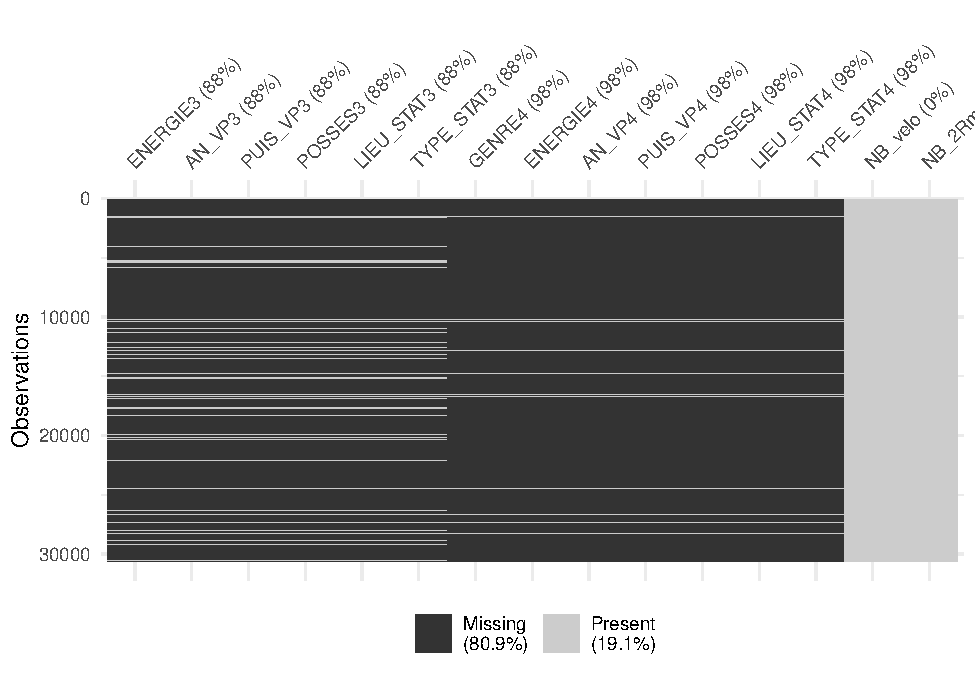
\includegraphics{Projet_Flo_2_files/figure-latex/unnamed-chunk-16-1.pdf}

\emph{Listes variables à plus de 80\% de valeurs manquantes}

-motoracc -situveil -STAT\_TRAV -TYPE\_STAT4 -LIEU\_STAT4 -POSSES4
-PUIS\_VP4 -AN\_VP4 -ENERGIE4 -GENRE4 -TYPE\_STAT3 -LIEU\_STAT3 -POSSES3
-PUIS\_VP3 -AN\_VP3 -ENERGIE3 -motdeacc -nbarret -abonpeage

\end{document}
